\documentclass[a4paper]{article}

%% Language and font encodings
\usepackage[french]{babel}
\usepackage[utf8x]{inputenc}
\usepackage[T1]{fontenc}

%% Sets page size and margins
\usepackage[a4paper,top=3cm,bottom=3cm,left=2cm,right=2cm,marginparwidth=2cm]{geometry}

%% Useful packages
\usepackage{amsmath}
\usepackage{graphicx}
\usepackage[colorinlistoftodos]{todonotes}
\PassOptionsToPackage{hyphens}{url}
\usepackage[colorlinks=true, allcolors=black]{hyperref}
\usepackage{fourier-orns}
\usepackage{titlesec}
\usepackage{fancyhdr}
\usepackage{fancyvrb}
\pagestyle{fancy}
\setcounter{tocdepth}{5}

%% Pour les exemples
\usepackage{mdframed}
\newmdenv[topline=false, bottomline=false, rightline=false, skipabove=\topsep, skipbelow=\topsep]{example}

%% Tikz stuff
\usepackage{tikz}
\usetikzlibrary{calc, arrows}
\tikzstyle{incolore} = [rectangle, rounded corners, draw=black, minimum height=1cm, minimum width=3cm, text width=3cm, text centered]

\usepackage{libertine}
\newcommand{\hsp}{\hspace{20pt}}
\newcommand{\HRule}{\rule{\linewidth}{0.5mm}}

\renewcommand{\headrulewidth}{1pt}
\fancyhead[C]{} 
\fancyhead[L]{}
\fancyhead[R]{\footnotesize{\leftmark}}

\renewcommand{\footrulewidth}{1pt}
\fancyfoot[C]{} 
\fancyhead[L]{}
\fancyfoot[R]{\thepage}

\definecolor{Zgris}{rgb}{0.87,0.85,0.85}

\usepackage{eso-pic,graphicx}
\usepackage{xcolor}
\newcommand{\bgimg}[1]
{
    \AddToShipoutPicture
    {
        \put(\LenToUnit{0 cm},\LenToUnit{0 cm})
        {
            \includegraphics[width=\paperwidth,height=\paperheight]{#1}
        }
    }
}

%% To list and caption code
\usepackage{minted}
\renewcommand{\listoflistingscaption}{Table des programmes}
\usepackage{caption}
\newenvironment{code}{\captionsetup{type=listing}}{}
\renewcommand{\listingscaption}{Programme}

\begin{document}




\begin{titlepage}
    \begin{sffamily}
        \begin{center}

            
\includegraphics[width=5cm]{images/LogoHenallux.PNG}~\\[1.5cm]
            \textsc{\Large Rapport de laboratoire}\\[1.5cm]

            \HRule \\[0.4cm]
            { \huge \bfseries Manipulation 1 : Metadata\\[0.4cm] }
            \HRule \\[2cm]

            \begin{minipage}{0.4\textwidth}
                \begin{flushleft} \large
                    Roumache Grégoire\\
                    Sénéchal Julien\\
                    Wallemme Maxime\\
                \end{flushleft}
            \end{minipage}
            \begin{minipage}{0.55\textwidth}
                \begin{flushright} \large
                    IR317 - Forensics and cyberattack evidence 2021-2022\\
                    Sécurité des systèmes, Hénallux\\
                    Troisième année, Classe A Groupe 1 \\
                \end{flushright}
            \end{minipage}
            \vfill

            {\large 28 Octobre 2021}

        \end{center}
    \end{sffamily}
\end{titlepage}

\let\cleardoublepage\clearpage















\section{Introduction}

Dans le cadre de ce laboratoire, nous avons dû identifier le suspect d'un crime cyber à l'aide d'outils forensics et OSINT à partir de l'image de la clé USB utilisée pour commettre le crime et des logs de l'ordinateur victime. Nous l'avons fait en quatre étapes : la mise en place de l'environnement, l'identification du suspect à partir de la clé USB, la recherche de fichiers susceptibles d'avoir été utilisés ou transférés et la vérification du disque en fin d'analyse.














\section{Mise en place de l'environnement}

\begin{enumerate}
    \item Nous avons calculé le hash de l'image afin de prouver qu'aucune modification n'a été apportée à celle-ci durant l'analyse \emph{(voir Figure \ref{hash_begining})}.
    \begin{figure}[H]
        \centering
        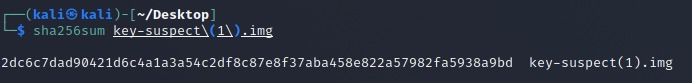
\includegraphics[width=15cm]{images/0.1) hash.PNG}
        \caption{Calcul du hash de l'image}
        \label{hash_begining}
    \end{figure}
    
    \item Nous avons ensuite du vérifier la taille de l'image et la notée car il s'agit d'une information importante lors du montage \emph{(voir Figure \ref{check_width})}.
    \begin{figure}[H]
        \centering
        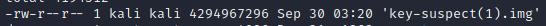
\includegraphics[width=15cm]{images/1) taille.PNG}
        \caption{Vérification de la taille de l'image}
        \label{check_width}
    \end{figure}
    
    \item Pour le calcul de l'offset, nous avons dû trouver le secteur de démarrage \emph{(voir Figure \ref{start_sector})}, et le multiplier par 512 car une unité est égal à 1 * 512, ce qui nous donne \emph{1048576}. Pour l'option sizelimit lors du montage de l'image, nous devons effectué le même calcul mais avec le secteur de fin ici égal à 8384512, ce qui donne 8384512 * 512 = 4292870144.
    \begin{figure}[H]
        \centering
        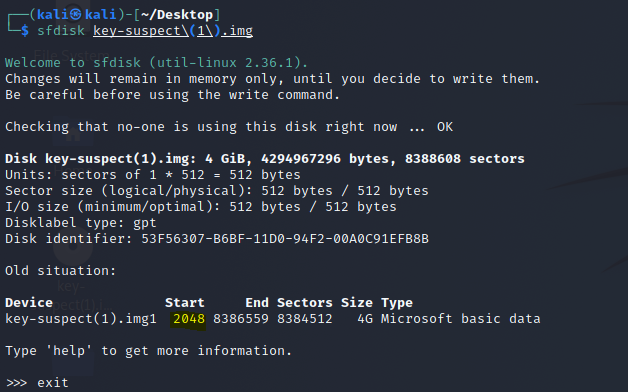
\includegraphics[width=11cm]{images/2) calcul_offset.PNG}
        \caption{Calcul de l'offset}
        \label{start_sector}
    \end{figure}
    
    \item Pour le montage, il nous a fallut tout d'abord associer l'image à un "device". Pour cela, nous avons utilisé la commande \emph{losetup} afin d'associer le "périphérique" /dev/loop0 à notre image. Ensuite, il nous a simplement fallut monter notre image comme pour n'importe quel périphérique tout en spécifiant les différentes options (Read-only, offset, sizelimit, ...). Au début, nous avons tous les trois montés notre image sans utiliser l'option du Read-Only. Ensuite, ayant déjà effectué des actions sur l'image de la clé usb, cela modifiait le hash de base obtenu plus haut, ce qui lors d'une enquête par exemple peut fausser les preuves. Nous avons alors démonté l'image pour la remonter avec l'option "ro" pour read-only.  \emph{(voir Figure \ref{mount})}. Grâce à l'option "Read-Only", nous avons la certitude de ne pas modifier notre image disque.

\begin{figure}[H]
    \centering
    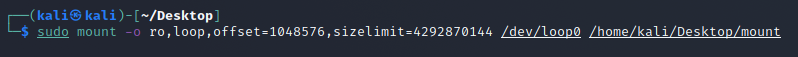
\includegraphics[width=15cm]{images/3) montage en read-only.PNG}
    \caption{Calcul de l'offset}
    \label{mount}
\end{figure}
    
\end{enumerate}



%%















\section{Identification du suspect}

Ayant accès maintenant à l’image sans risquer aucune modification, nous commençons par chercher une preuve permettant d’identifier le suspect décrit par le vigile.

Après plusieurs recherches au sein des dossiers et fichiers contenus dans la clé USB, nous avons trouvé un dossier caché à la source de la clé USB. Il s’agit du dossier .Trash-1000 correspondant au dossier de la corbeille. Lorsque l’on supprime un élément du disque, celui-ci est déplacé dans la corbeille et donc dans ce dossier. Il contient un dossier tweets, supprimé par le suspect, qui lui-même contient quatre fichiers « .png ».

\begin{figure}[H]
    \centering
    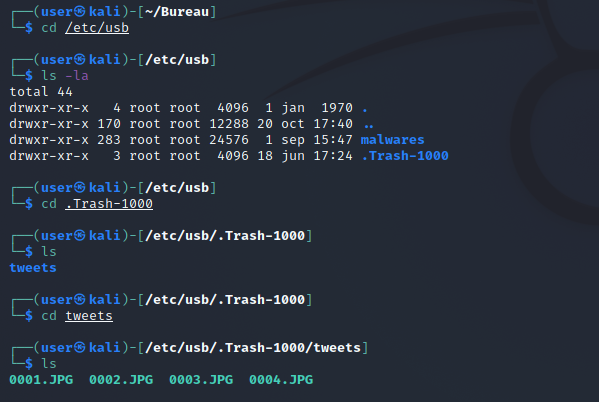
\includegraphics[width=15cm]{images/Fichiers caches cle usb.png}
    \caption{Fichiers cachés sur la clé usb}
    \label{hidden_files}
\end{figure}

En examinant les photos, on remarque que l’une des personnes présente sur deux des images correspond à la description du suspect donnée par le vigile.

    
\begin{figure}[H]
    \centering
    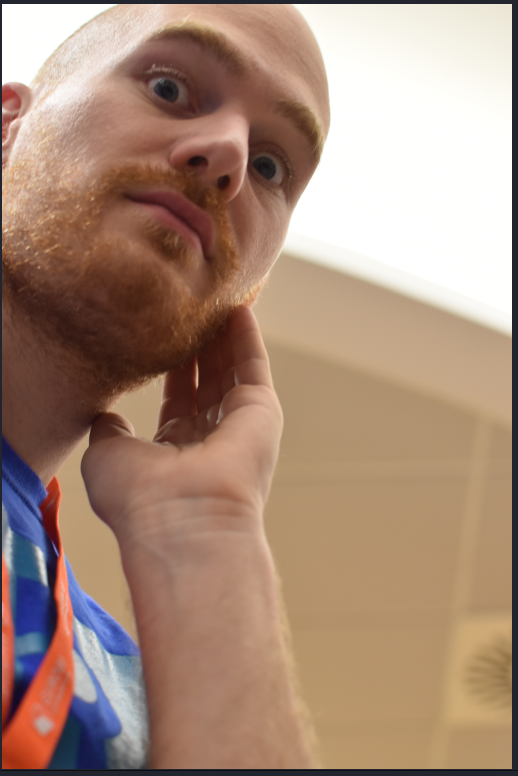
\includegraphics[width=7cm]{images/Photo 2 cle usb.png}
    \caption{Photo n°1 trouvée dans le dossier caché}
    \label{first_picture}
\end{figure}
    
\begin{figure}[H]
    \centering
    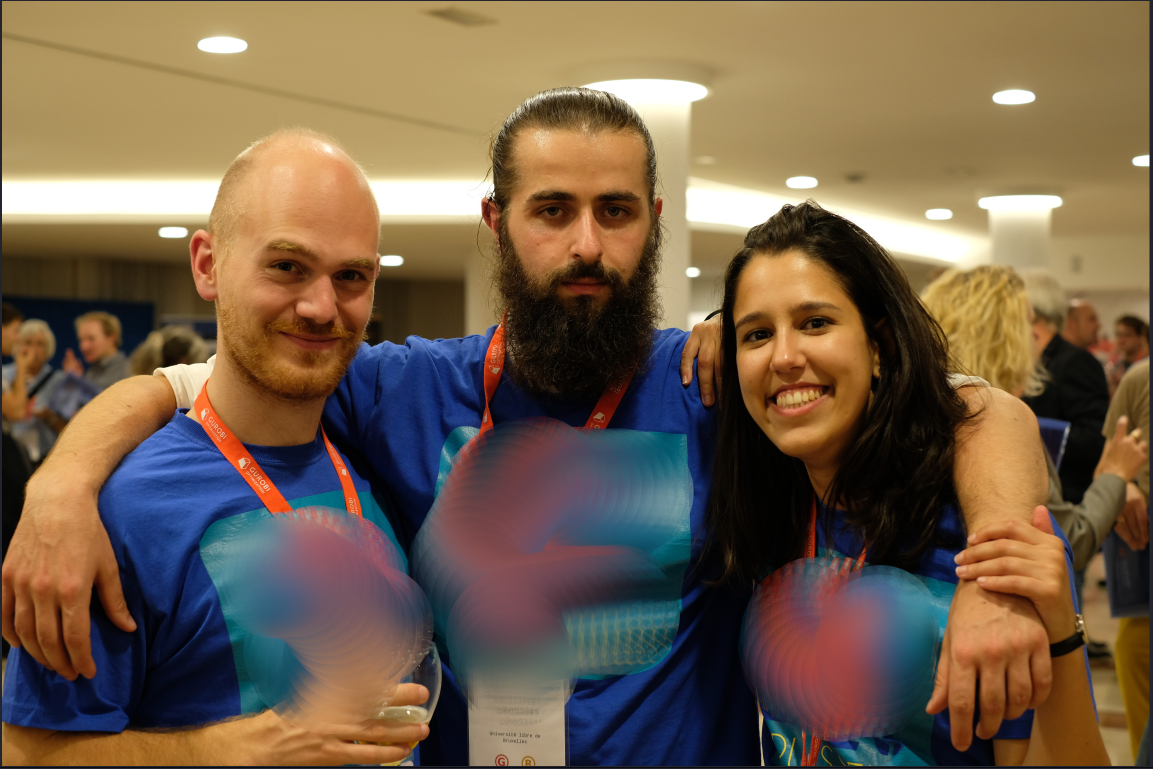
\includegraphics[width=10cm]{images/Photo 3 cle usb.png}
    \caption{Photo n°2 trouvée dans le dossier caché}
    \label{second_picture}
\end{figure}


On peut également voir d’autres personnes présentent sur les photos. On remarque aussi qu'elles ont été prises lors d’un évènement ressemblant à une conférence.
Notre objectif maintenant est donc de pouvoir trouver plus d’informations sur ces personnes et sur l’évènement afin d’identifier correctement le suspect.

\begin{figure}[H]
    \centering
    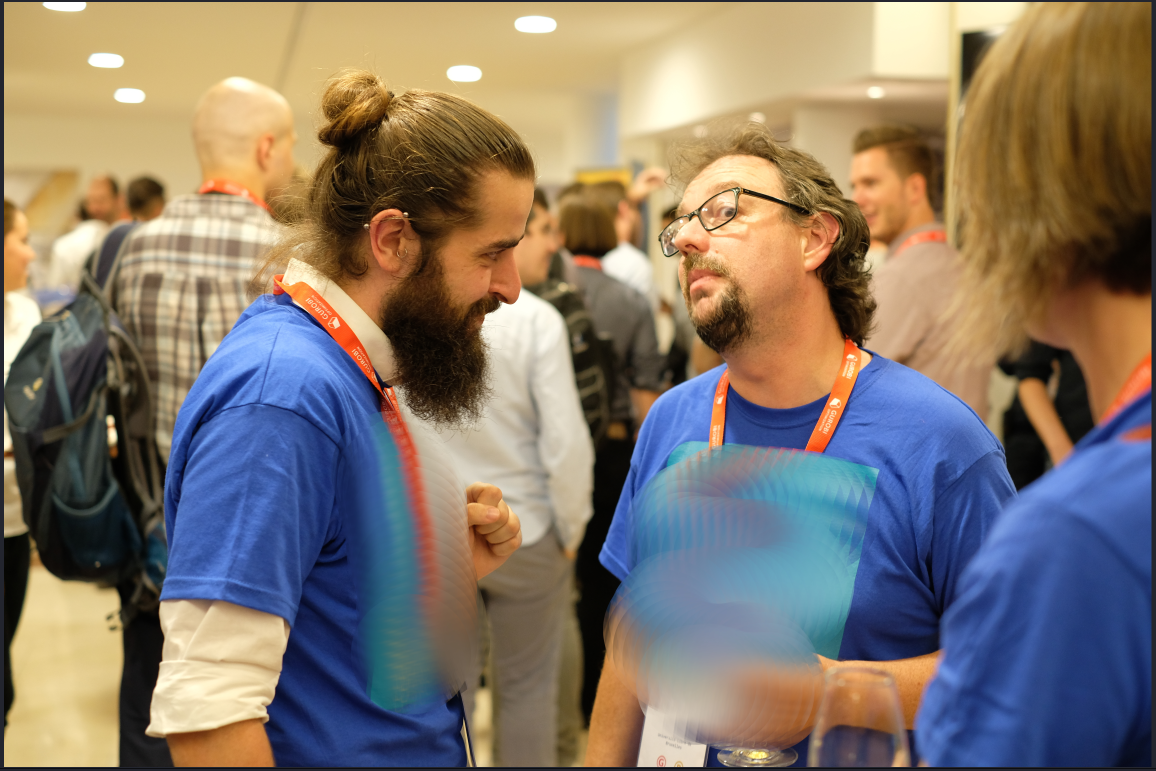
\includegraphics[width=10cm]{images/Photo 1 cle usb.png}
    \caption{Photo n°3 trouvée dans le dossier caché}
    \label{third_picture}
\end{figure}

\begin{figure}[H]
    \centering
    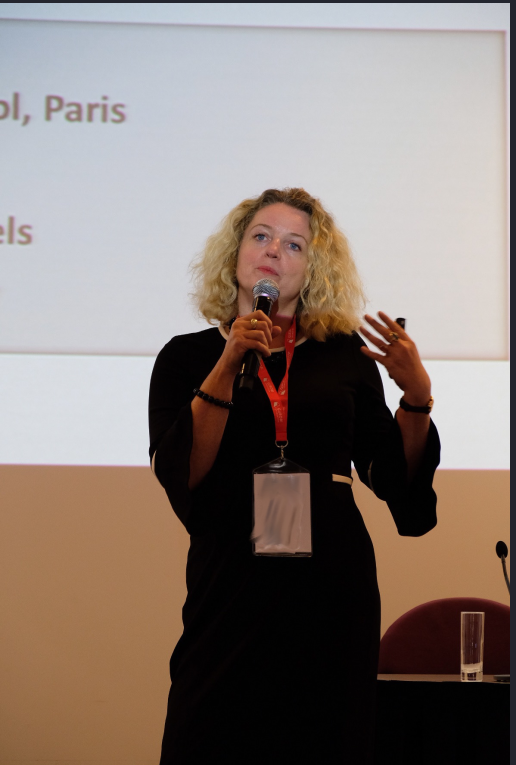
\includegraphics[width=6cm]{images/Photo 4 cle usb.png}
    \caption{Photo n°4 trouvée dans le dossier caché}
    \label{fourth_picture}
\end{figure}


Premièrement, nous pouvons identifier l’une des personnes présente sur 2 photos parmi les 5. Il s’agit de Guillerme Duvillié, notre professeur.

Ensuite, nous analysons les metadonnées des images à l’aide de la commande exiftool.
Nous obtenons alors plusieurs informations intéressantes :
\begin{itemize}
    \item Nom du photographe : Frank Plein
    \item Date de création de la photo : 11 septembre 2018
    \item Des coordonnées GPS : 50° 49' 25.79"  4° 21' 40.25"\\
    Ceci nous amène au MCE (Management Centre Europe)
\end{itemize}
\newpage
Après avoir obtenu ces quelques premières informations, nous essayons d’identifier le suspect à l’aide d’une des photos et de l’outil en ligne Pineyes.
Malheureusement, aucun résultat concluant n’en ressort.

Nous poursuivons nos recherches sur internet avec le nom du photographe.
Nous essayons de chercher des informations via les réseaux sociaux, nous obtenons alors un profil twitter. Sur celui-ci, nous trouvons une photo sur laquelle se trouve une personne ressemblant fortement au suspect, Mathieu Besançon. Dans la publication, cette personne est identifiée, nous avons donc accès à son twitter.

\begin{figure}[H]
    \centering
    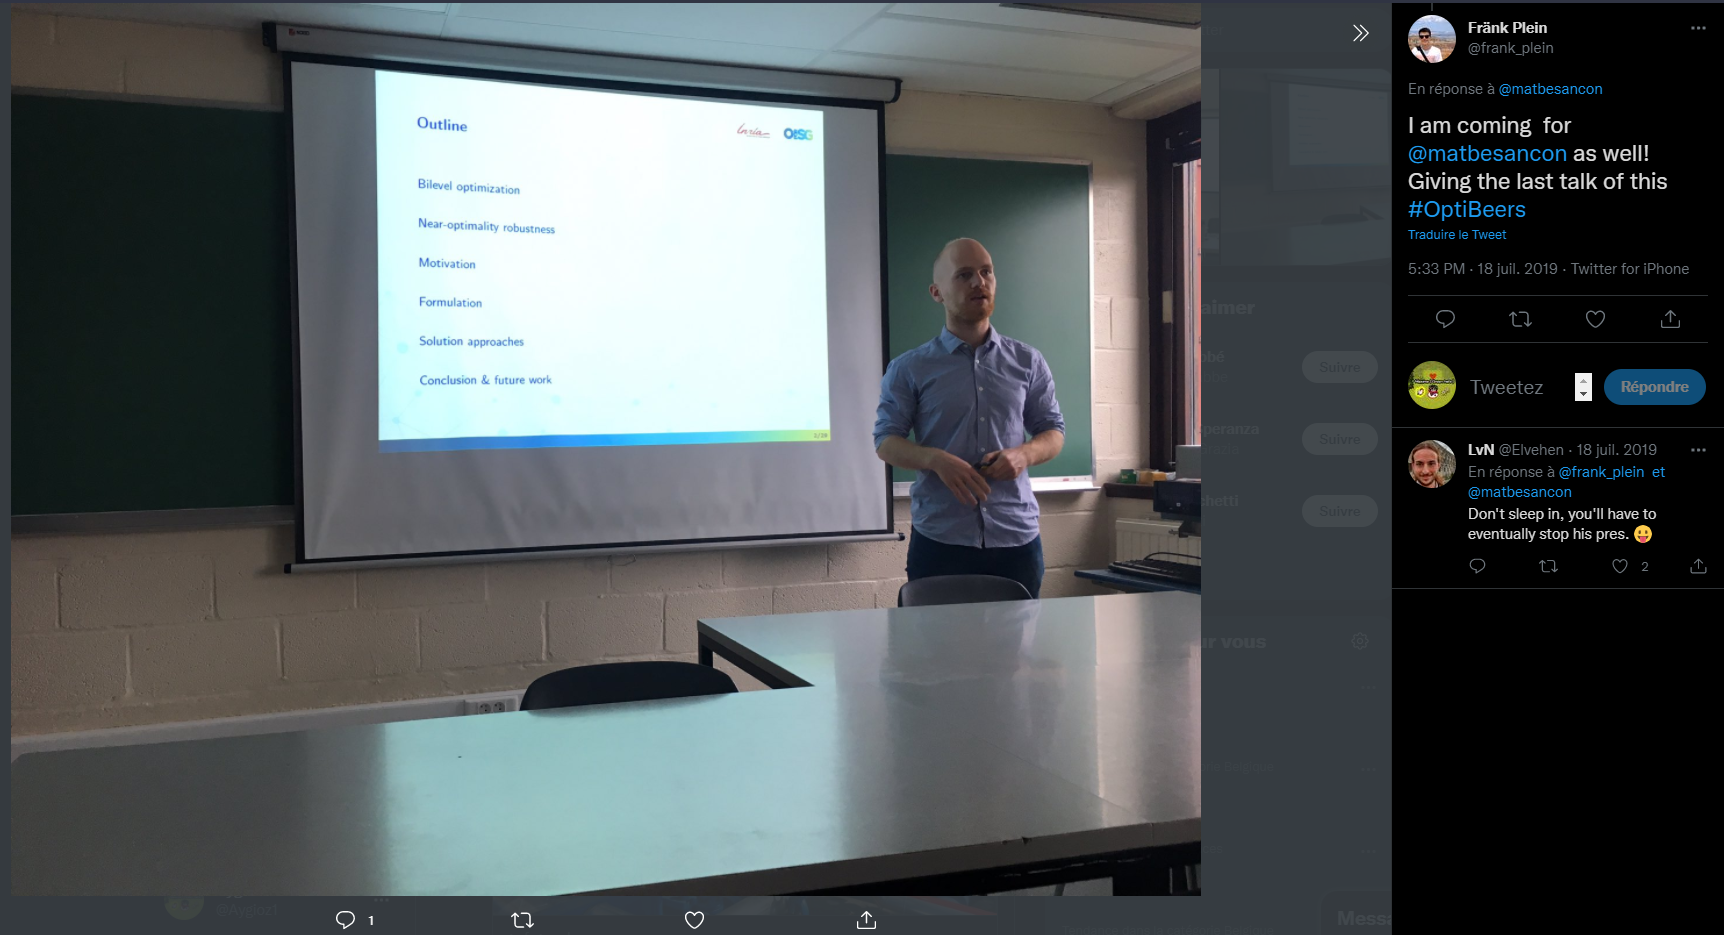
\includegraphics[width=10cm]{images/Twitter du supect via Frank Plein.png}
    \caption{Possible profil du suspect identifié via Frank Plein}
    \label{possible_twitter_profile}
\end{figure}

Mais nous ne savons pas s’il s’agit bien de la personne que l’on cherche.

Sur le twitter de Frank Plein, nous trouvons une vieille publication datant du 10 septembre 2018.
La date de cette publication est proche de la date de création des photos obtenues dans l’analyse des métadonnées.
Cette publication contient également une photo sur laquelle on peut clairement identifier le suspect, Guillerme Duvillie et une troisième personne qui sont présentes sur les photos trouvées sur l’image de la clé usb.
Mais aussi, on remarque que les t-shirts et les tours de cou sont ressemblants à ceux que portent les personnes sur les images trouvées. De plus, le logo \emph{MCE} est affiché sur le mur, ce qui nous confirme qu'il s'agit du même évènement.

\begin{figure}[H]
    \centering
    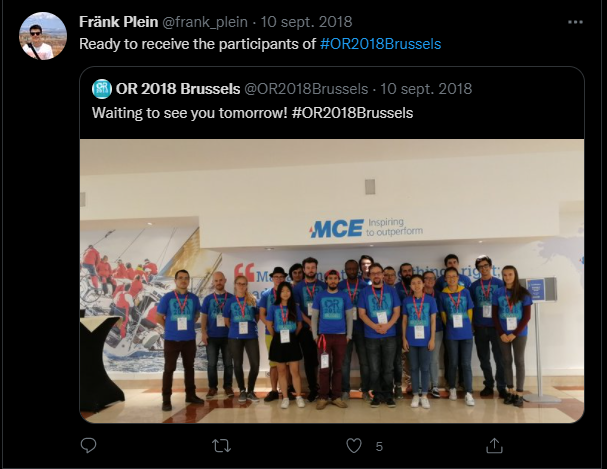
\includegraphics[width=10cm]{images/Publication de Frank Plein sur la conf.png}
    \caption{Identification de la conférence}
    \label{conference}
\end{figure}

Via cette publication, nous obtenons le nom et le compte twitter de la conférence.
Il s’agit de OR2018Brussels.
En remontant les publications du compte twitter de la conférence, nous identifions une troisième personne. 
Il s’agit cette fois de Ivana Ljubic que nous identifions grâce à des photos similaires à celles trouvées sur la clé usb.

\begin{figure}[H]
    \centering
    
\includegraphics[width=8cm]{images/Identification personne 3.png}
    \caption{Identification de la personne n°3 depuis le twitter de la conférence}
    \label{identity_third_person}
\end{figure}

A l’aide de deux autres publications, nous identifions une quatrième personne, Bernard Fortz.

\begin{figure}[H]
    \centering
    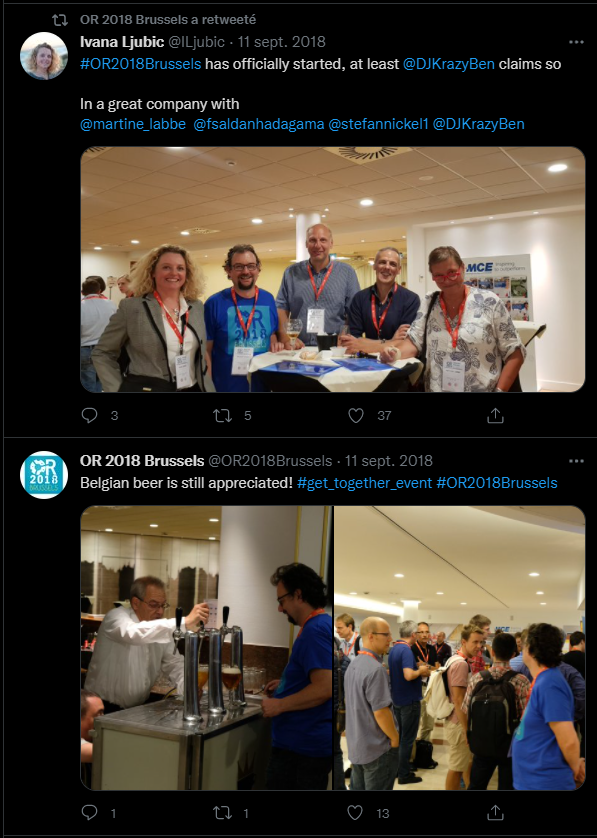
\includegraphics[width=9cm]{images/Identification personne 4.png}
    \caption{Identification de la personne n°4 depuis le twitter de la conférence}
    \label{identity_fourth_person}
\end{figure}

Ne trouvant plus aucun autre indice, nous décidons d’explorer en détails les comptes Twitter des deux dernières personnes identifiées.

En remontant le fil d’actualité du compte de Bernard Fortz, nous trouvons une publication, qu’il a retweeté, venant du compte twitter de Mathieu Besançon. Il s’agit du même compte que nous avons pu trouver lorsque nous avons examiné le profil de Frank Plein. Cette publication trouvée, parle da la conférence OR2018Brussels et sa date corresponds aux dates trouvées dans les métadonnées. 

\begin{figure}[H]
    \centering
    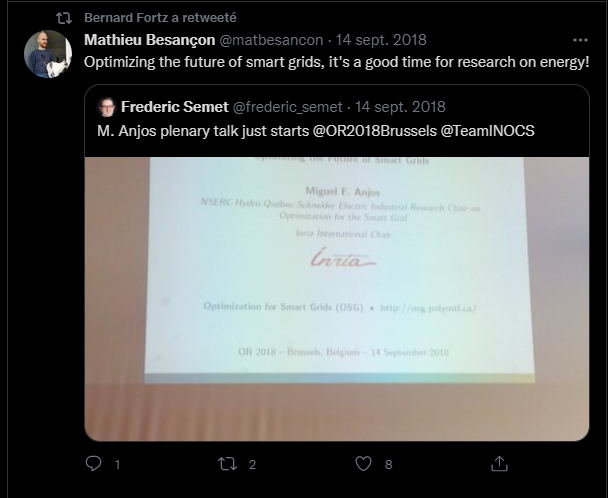
\includegraphics[width=9cm]{images/Identification suspect.png}
    \caption{Identification du suspect via le profil de Bernard Fortz}
    \label{identity_bernard_fortz}
\end{figure}

Nous pouvons alors affirmer que cette personne trouvée est bien le suspect que nous recherchons.
Il s’agit donc de Mathieu Besançon, son profil twitter est @matbesancon.

\begin{figure}[H]
    \centering
    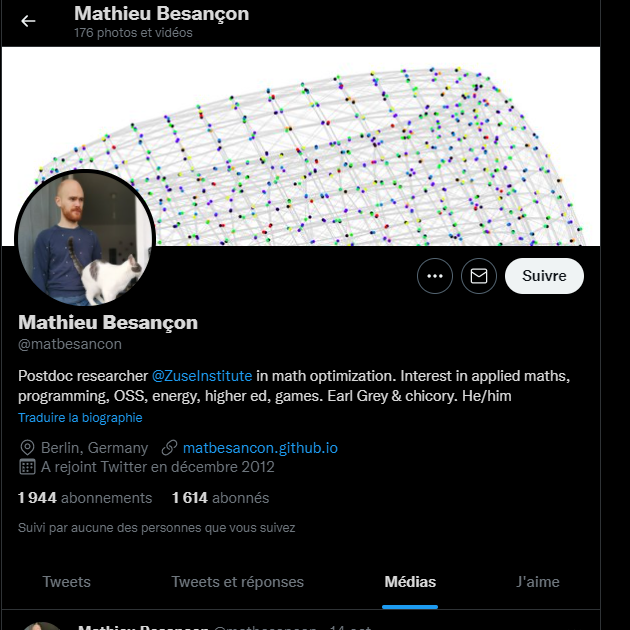
\includegraphics[width=10cm]{images/Twitter du suspect.png}
    \caption{Profil twitter du suspect}
    \label{twitter_profile}
\end{figure}


%%















\section{Recherche des fichiers susceptibles d'avoir été utilisés ou transférés}





\subsection{Analyse des logs}

Nous avons un fichier d'événements Windows au format \textit{Event Log Format} (evtx). Nous pouvons utiliser l'application \textit{Observateur d'événements} sur Windows pour l'analyser mais c'est beaucoup plus facile d'utiliser une plateforme comme Splunk. Comme c'est possible d'utiliser Splunk avec un conteneur Docker, il n'y a pas besoin de l'installer, nous pouvons simplement utiliser les commandes suivantes :
\begin{example}
\begin{Verbatim}[fontsize=\small]
$ docker pull splunk/splunk:latest
$ docker run -d -p 8000:8000 -e "SPLUNK_START_ARGS=--accept-license" \
    -e "SPLUNK_PASSWORD=test1234" --name splunk splunk/splunk:latest
\end{Verbatim}
\end{example}
Nous y accédons ensuite via une interface web en allant sur {\small \url{http://localhost:8000/}} et en utilisant les identifiants \textit{admin} et \textit{test1234}.

Malheureusement, nous ne pouvons pas utiliser l'analyseur d'événements dans ce format sans ajouter une extension. Nous pouvons cependant modifier le format en CSV avec l'outil \textit{Log Parser} \cite{1} de Microsoft. Une fois installé, nous utilisons la commande suivante :
\begin{example}
\begin{Verbatim}[fontsize=\small]
$ LogParser "Select * INTO logAttaque.csv FROM logAttaque.evtx" -i:evt -o:csv
\end{Verbatim}
\end{example}

En filtrant en fonction de la date (le 19 septembre 2021), nous obtenons 983 événements, 50 \textit{Event ID} différents et 11 \textit{Source Name} différents. Nous avons commencé en essayant de réduire le nombre d'événements à analyser en excluant des \textit{Event ID} non-pertinents. Comme il y en avait beaucoup, on risquait d'y perdre des heures. Ensuite, nous avons remarqué qu'on pouvait filtrer sur la catégorie \textit{Source Name}. La seule valeur pertinente étant \textit{Microsoft-Windows-DriverFrameworks-UserMode}, nous avons utilisé la requête Splunk suivante :
\begin{example}
\begin{Verbatim}[fontsize=\small]
SourceName="Microsoft-Windows-DriverFrameworks-UserMode"
\end{Verbatim}
\end{example}
Il ne nous reste alors plus que 67 événements et 16 \textit{Event ID} différents. À ce moment dans l'analyse, nous avons pensé que c'était une bonne idée de chercher plus d'informations sur l'analyse de logs en cas d'attaque via une clé USB. Nous avons donc trouvé les informations suivantes \cite{2} :
\begin{itemize}
    \item Filtrer les \textit{Event ID} 1003, 2000, 2001, 1004, pour trouver quelle clé USB a été utilisée et à quelle heure le 19 septembre 2021 et quels processus sont ouverts. Ensuite, nous pouvons regarder quand ces processus sont fermés pour trouver quand la clé USB a été retirée.
    \begin{enumerate}
        \item Processus 50275a46-0018-4ca9-9c87-e9cd6ca0d441 à 19-09-21 15:43:07.
        \item Processus 17e60a64-4493-4d32-8586-0b0a1b71302f à 19-09-21 15:45:18.
        \item Processus 9b7a213b-cbe9-4db2-ab90-9d16b485522b à 19-09-21 15:50:16.
    \end{enumerate}
    \item Filtrer les \textit{Event ID} 1006, 2900, 2901, 1008, pour trouver quand la clé USB a été retirée.
    \begin{enumerate}
        \item Processus jamais tué...
        \item Processus 17e60a64-4493-4d32-8586-0b0a1b71302f à 19-09-21 15:50:08.
        \item Processus 9b7a213b-cbe9-4db2-ab90-9d16b485522b à 19-09-21 16:06:07.
    \end{enumerate}
\end{itemize}
Grâce à l'Event ID 1003, nous avons pu identifier l'UUID de la clé USB qui a été connecté. Nous obtenons l'UUID suivant :
\begin{example}
\begin{Verbatim}[fontsize=\small]
    53F56307-B6BF-11D0-94F2-00A0C91EFB8B
\end{Verbatim}
\end{example}
Il nous faut alors vérifier que celui-ci correspond bien à l'UUID de l'image de la clé que nous analysons. Pour cela, nous nous rendons sur Linux et grâce à la commande \emph{blkid} nous obtenous l'UUID de notre image. Celle-ci correspond bien à l'UUID rencontré dans nos logs (\emph{voir Figure \ref{key_analysis}} ).

\begin{figure}[H]
    \centering
    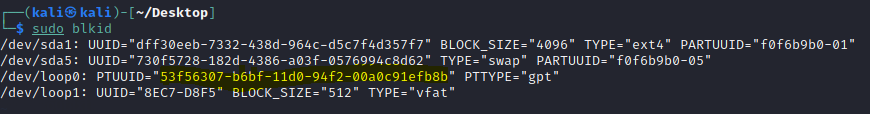
\includegraphics[width=16cm]{images/UUID-key.PNG}
    \caption{UUID de la clé analysée}
    \label{key_analysis}
\end{figure}

Maintenant que nous avons l'UUID, nous pouvons vérifier si cette même clé fut connecté d'autres jours que le 19 septembre. Nous retirons donc le filtre de date sur notre Event Viewer et nous resserrons les Event ID nous intéressant au 1003 uniquement. En regardant les détails des logs affichés, nous pouvons constater que la clé à non seulement été connecté le 19 septembre, mais également le 16 et le 22 septembre (\emph{Voir Figure \ref{differents_days}} ).

\begin{figure}[H]
    \centering
    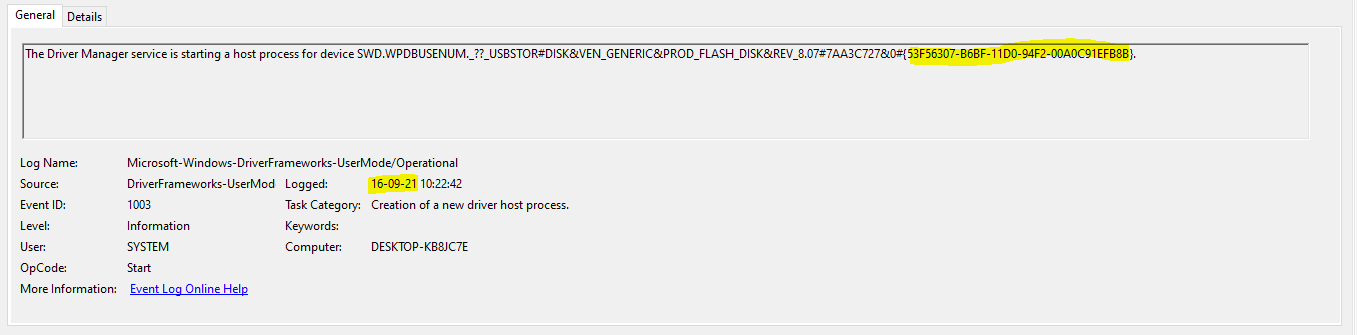
\includegraphics[width=15cm]{images/key-usb-16-09.PNG}\\
    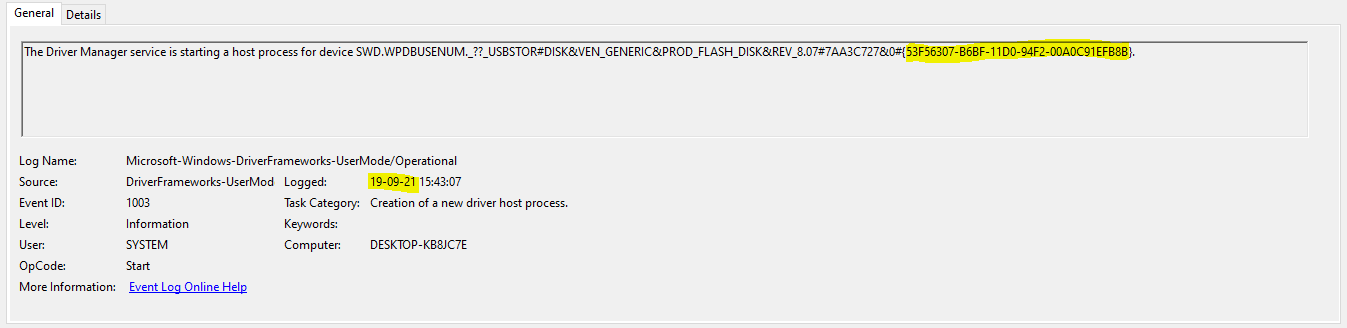
\includegraphics[width=15cm]{images/key-usb-19-09.PNG}\\
    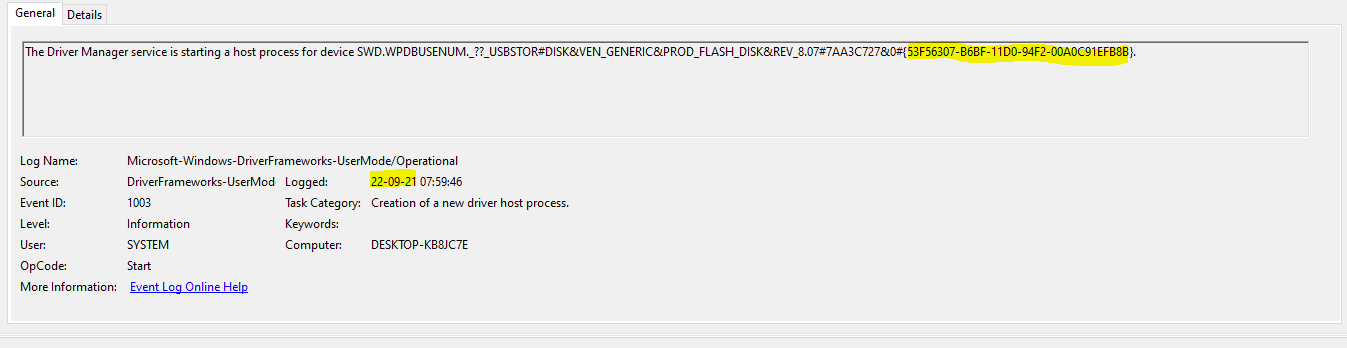
\includegraphics[width=15cm]{images/key-usb-22-09.PNG}\\
    \caption{Connections de la clé différents jours - Logs Details}
    \label{differents_days}
\end{figure}





\subsection{Identification des fichiers copiés}

Étant donné que nous savons que la clé fut branchée au poste de travail le 16, 19 et 22 septembre; il nous faut maintenant retrouver les fichiers ayant été possiblement copié voir modifié ! Pour cela, il a fallut tout d'abord remettre notre machine de travail dans le même environnement que celui du poste de travail du CHR, ce que nous avons fait grâce à NTP. Après cela, il nous a suffit de retrouver les fichier ayant été modifié à ces dates grâce aux timestamps de ceux-ci. Malheureusement, aucun fichier n'avait de timestamp de modification qui correspondait à ces dates. Nous avons donc vérifié à nouveau, mais cette fois-ci pour les timestamp d'\emph{accès} au fichier. Nous avons ainsi pu trouver une série de fichiers ayant été copiés durant ces dates comme vous pouvez le voir sur la figure \ref{copied_files}. Malheureusement, il nous est impossible de savoir à quel heure on a accédé à ces fichiers. Nous avons effectué cette recherche grâce au script python ci-dessous :
\begin{code}\small
\begin{minted}[xleftmargin=20pt,linenos]{python}
import os
import stat
import sys
import time

dir = sys.argv[1]

for root, directories, files in os.walk(dir):
    for file in files:
        full_path = os.path.join(root, file)
        stats_file = os.stat(full_path)
        access_time = time.ctime(stats_file [ stat.ST_ATIME ])

        if ("Sun Sep 19" in access_time or 
            "Thu Sep 16" in access_time or
            "Wed Sep 22" in access_time):
            
            print(access_time, full_path)
\end{minted}
\caption{Recherche des fichiers en fonction des heures d'accès}
\end{code}

\begin{figure}[H]
    \centering
    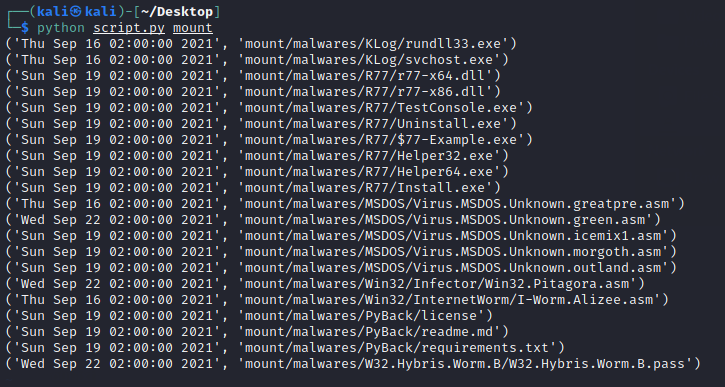
\includegraphics[width=15cm]{images/filemodified.PNG}
    \caption{Série de fichiers copiés}
    \label{copied_files}
\end{figure}


%%














\section{Vérification du disque en fin d'analyse}

Une fois l'analyse terminée, vient le moment de tout démonter et de vérifier que l'image n'a pas été altérée. Pour cela, nous procédons simplement a un \emph{umount}, puis nous dissocions notre image de notre device /dev/loop0 grâce à l'option \emph{-d} de losetup. Ne nous reste plus que recalculer le hash de notre image et de comparer celui-ci avec celui calculé en début de manipulation. Nous constatons que les hash sont bel et bien identique ce qui signifie que rien n'a été modifié dans l'image \emph{(voir Figure \ref{hash_ending})}.

\begin{figure}[H]
    \centering
    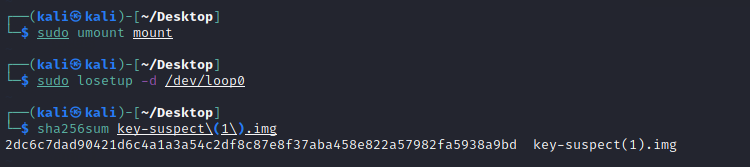
\includegraphics[width = 15cm]{images/fin.PNG}
    \caption{Calcul du hash en fin d'analyse}
    \label{hash_ending}
\end{figure}




%%














\newpage
\section{Conclusion}





%Lors de cette série de deux laboratoires, nous nous sommes d'abord bien amusé. C'était très amusant de chercher l'identité de quelqu'un à partir de sa photo sans autre information. De même pour la partie forensics, la recherche n'a pas été facile mais très riche en apprentissage. C'était notre première expérience d'OSINT et de forensics, et nous en sortons avec de meilleures connaissances sur les deux sujets, mais surtout, sur les métadonnées. Nous avons eu besoin des métadonnées internes pour la recherche OSINT et des métadonnées externes pour la partie forensics du laboratoire. Bien que nous ayons eu besoin d'analyser les logs et de faire des recherches sur internet, c'est les métadonnées qui ont été le coeur de ce laboratoire et nous en tirons une leçon pour l'avenir : pour identifier un suspect et son mode d'attaque, il faut regarder les métadonnées !

Tout d'abord, la mise en place de l'environnement de travail nous a permis de pouvoir analyser la pièce à conviction dans un cadre permettant d'assurer l'intégrité des données. Ensuite, l'identification du suspect a pu se faire grâce aux diverses images supprimées sur le disque ainsi qu'à leurs metadonnées. Ces métadonnées nous ayant permis d'orienter nos recherches sur Twitter et ainsi de retrouver le suspect. Enfin, les logs nous ont étés très utiles afin d'identifier les fichiers ayant étés possiblement copiés sur la machine cible.




















\appendix




















\section{Métadonnées}





\subsection{Définition de métadonnée}

Tout d'abord, qu'est-ce qu'une donnée ? Une donnée est la représentation informatique d'une information, par exemple une image ou un fichier texte stocké sur un ordinateur. Une métadonnée est une donnée sur une donnée, c'est-à-dire que c'est une donnée qui donne des informations sur une autre donnée, par exemple la date de création d'un fichier, l'auteur d'une photographie, etc.





\subsection{Différence entre des métadonnées internes et externes}

Certaines métadonnées sont stockées dans le fichier lui-même, un peu à l'image des commentaires python, elles ne sont pas toujours nécessaires à l'utilisation du fichier par le système (ex : avoir l'auteur d'une photographie dans les métadonnées ne permet pas de mieux voir l'image) mais elles peuvent donner de précieuses informations sur celui-ci.

Les métadonnées externes sont souvent générées par le système de fichier et permettent de savoir à qui appartient le fichier, quels accès les utilisateurs du système peuvent avoir dessus, à quelle date le fichier a été créé, etc.




\subsection{Quel genre d'informations trouve-t-on dans les métadonnées ?}

On peut y trouver de nombreuses informations comme le nom du fichier, son auteur, les droits que les utilisateurs et groupes ont sur le fichier (par exemple, si il est exécutable ou pas). Pour des fichiers comme les photos et vidéos, on trouve aussi des informations comme la géolocalisation, l'appareil photo utilisé, le logiciel d'édition, etc. Dans les programmes exécutables, on peut trouver le compilateur qui a changé le code source en instructions exécutables, parfois la date de compilation, mais aussi l'architecture pour laquelle il a été optimisé, etc.





\subsection{Quelles sont les différentes dates retrouvées dans les métadonnées externes ?}

Sur les systèmes Linux, on trouve trois types de dates :
\begin{itemize}
    \item la date de création du fichier;
    \item la date de dernière écriture dans le fichier;
    \item la date de dernière lecture du fichier.
\end{itemize}





\subsection{Commandes permettant d'accéder aux métadonnées externes}

Une commande souvent utilisée pour obtenir des métadonnées externes est \texttt{\small stats}. Mais pour avoir un maximum de métadonnées, autant internes qu'externes, on peut utiliser un meilleur outil \texttt{\small exiftool}.




















\newpage \tableofcontents \listoffigures \listoflistings
\begin{thebibliography}{9}
\bibitem{1} {\small \url{https://www.microsoft.com/en-us/download/details.aspx?id=24659}}
\bibitem{2} {\small \url{https://forensixchange.com/posts/19\_08\_03\_usb\_storage\_forensics\_1/}}
\bibitem{3} {\small \url{https://www.x-ways.net/winhex/manual.pdf}}
% \bibitem{4} 
% \bibitem{5} 
% \bibitem{6} 
\end{thebibliography}




















\end{document}
